% Options for packages loaded elsewhere
\PassOptionsToPackage{unicode}{hyperref}
\PassOptionsToPackage{hyphens}{url}
\documentclass[
]{book}
\usepackage{xcolor}
\usepackage{amsmath,amssymb}
\setcounter{secnumdepth}{5}
\usepackage{iftex}
\ifPDFTeX
  \usepackage[T1]{fontenc}
  \usepackage[utf8]{inputenc}
  \usepackage{textcomp} % provide euro and other symbols
\else % if luatex or xetex
  \usepackage{unicode-math} % this also loads fontspec
  \defaultfontfeatures{Scale=MatchLowercase}
  \defaultfontfeatures[\rmfamily]{Ligatures=TeX,Scale=1}
\fi
\usepackage{lmodern}
\ifPDFTeX\else
  % xetex/luatex font selection
\fi
% Use upquote if available, for straight quotes in verbatim environments
\IfFileExists{upquote.sty}{\usepackage{upquote}}{}
\IfFileExists{microtype.sty}{% use microtype if available
  \usepackage[]{microtype}
  \UseMicrotypeSet[protrusion]{basicmath} % disable protrusion for tt fonts
}{}
\makeatletter
\@ifundefined{KOMAClassName}{% if non-KOMA class
  \IfFileExists{parskip.sty}{%
    \usepackage{parskip}
  }{% else
    \setlength{\parindent}{0pt}
    \setlength{\parskip}{6pt plus 2pt minus 1pt}}
}{% if KOMA class
  \KOMAoptions{parskip=half}}
\makeatother
\usepackage{color}
\usepackage{fancyvrb}
\newcommand{\VerbBar}{|}
\newcommand{\VERB}{\Verb[commandchars=\\\{\}]}
\DefineVerbatimEnvironment{Highlighting}{Verbatim}{commandchars=\\\{\}}
% Add ',fontsize=\small' for more characters per line
\usepackage{framed}
\definecolor{shadecolor}{RGB}{248,248,248}
\newenvironment{Shaded}{\begin{snugshade}}{\end{snugshade}}
\newcommand{\AlertTok}[1]{\textcolor[rgb]{0.94,0.16,0.16}{#1}}
\newcommand{\AnnotationTok}[1]{\textcolor[rgb]{0.56,0.35,0.01}{\textbf{\textit{#1}}}}
\newcommand{\AttributeTok}[1]{\textcolor[rgb]{0.13,0.29,0.53}{#1}}
\newcommand{\BaseNTok}[1]{\textcolor[rgb]{0.00,0.00,0.81}{#1}}
\newcommand{\BuiltInTok}[1]{#1}
\newcommand{\CharTok}[1]{\textcolor[rgb]{0.31,0.60,0.02}{#1}}
\newcommand{\CommentTok}[1]{\textcolor[rgb]{0.56,0.35,0.01}{\textit{#1}}}
\newcommand{\CommentVarTok}[1]{\textcolor[rgb]{0.56,0.35,0.01}{\textbf{\textit{#1}}}}
\newcommand{\ConstantTok}[1]{\textcolor[rgb]{0.56,0.35,0.01}{#1}}
\newcommand{\ControlFlowTok}[1]{\textcolor[rgb]{0.13,0.29,0.53}{\textbf{#1}}}
\newcommand{\DataTypeTok}[1]{\textcolor[rgb]{0.13,0.29,0.53}{#1}}
\newcommand{\DecValTok}[1]{\textcolor[rgb]{0.00,0.00,0.81}{#1}}
\newcommand{\DocumentationTok}[1]{\textcolor[rgb]{0.56,0.35,0.01}{\textbf{\textit{#1}}}}
\newcommand{\ErrorTok}[1]{\textcolor[rgb]{0.64,0.00,0.00}{\textbf{#1}}}
\newcommand{\ExtensionTok}[1]{#1}
\newcommand{\FloatTok}[1]{\textcolor[rgb]{0.00,0.00,0.81}{#1}}
\newcommand{\FunctionTok}[1]{\textcolor[rgb]{0.13,0.29,0.53}{\textbf{#1}}}
\newcommand{\ImportTok}[1]{#1}
\newcommand{\InformationTok}[1]{\textcolor[rgb]{0.56,0.35,0.01}{\textbf{\textit{#1}}}}
\newcommand{\KeywordTok}[1]{\textcolor[rgb]{0.13,0.29,0.53}{\textbf{#1}}}
\newcommand{\NormalTok}[1]{#1}
\newcommand{\OperatorTok}[1]{\textcolor[rgb]{0.81,0.36,0.00}{\textbf{#1}}}
\newcommand{\OtherTok}[1]{\textcolor[rgb]{0.56,0.35,0.01}{#1}}
\newcommand{\PreprocessorTok}[1]{\textcolor[rgb]{0.56,0.35,0.01}{\textit{#1}}}
\newcommand{\RegionMarkerTok}[1]{#1}
\newcommand{\SpecialCharTok}[1]{\textcolor[rgb]{0.81,0.36,0.00}{\textbf{#1}}}
\newcommand{\SpecialStringTok}[1]{\textcolor[rgb]{0.31,0.60,0.02}{#1}}
\newcommand{\StringTok}[1]{\textcolor[rgb]{0.31,0.60,0.02}{#1}}
\newcommand{\VariableTok}[1]{\textcolor[rgb]{0.00,0.00,0.00}{#1}}
\newcommand{\VerbatimStringTok}[1]{\textcolor[rgb]{0.31,0.60,0.02}{#1}}
\newcommand{\WarningTok}[1]{\textcolor[rgb]{0.56,0.35,0.01}{\textbf{\textit{#1}}}}
\usepackage{longtable,booktabs,array}
\usepackage{calc} % for calculating minipage widths
% Correct order of tables after \paragraph or \subparagraph
\usepackage{etoolbox}
\makeatletter
\patchcmd\longtable{\par}{\if@noskipsec\mbox{}\fi\par}{}{}
\makeatother
% Allow footnotes in longtable head/foot
\IfFileExists{footnotehyper.sty}{\usepackage{footnotehyper}}{\usepackage{footnote}}
\makesavenoteenv{longtable}
\usepackage{graphicx}
\makeatletter
\newsavebox\pandoc@box
\newcommand*\pandocbounded[1]{% scales image to fit in text height/width
  \sbox\pandoc@box{#1}%
  \Gscale@div\@tempa{\textheight}{\dimexpr\ht\pandoc@box+\dp\pandoc@box\relax}%
  \Gscale@div\@tempb{\linewidth}{\wd\pandoc@box}%
  \ifdim\@tempb\p@<\@tempa\p@\let\@tempa\@tempb\fi% select the smaller of both
  \ifdim\@tempa\p@<\p@\scalebox{\@tempa}{\usebox\pandoc@box}%
  \else\usebox{\pandoc@box}%
  \fi%
}
% Set default figure placement to htbp
\def\fps@figure{htbp}
\makeatother
\setlength{\emergencystretch}{3em} % prevent overfull lines
\providecommand{\tightlist}{%
  \setlength{\itemsep}{0pt}\setlength{\parskip}{0pt}}
\usepackage[]{natbib}
\bibliographystyle{plainnat}
\usepackage{booktabs}
\usepackage{bookmark}
\IfFileExists{xurl.sty}{\usepackage{xurl}}{} % add URL line breaks if available
\urlstyle{same}
\hypersetup{
  pdftitle={A Minimal Book Example},
  pdfauthor={John Doe},
  hidelinks,
  pdfcreator={LaTeX via pandoc}}

\title{A Minimal Book Example}
\author{John Doe}
\date{2024-10-21}

\begin{document}
\maketitle

{
\setcounter{tocdepth}{1}
\tableofcontents
}
\chapter{About}\label{about}

This is a \emph{sample} book written in \textbf{Markdown}. You can use anything that Pandoc's Markdown supports; for example, a math equation \(a^2 + b^2 = c^2\).

\section{Usage}\label{usage}

Each \textbf{bookdown} chapter is an .Rmd file, and each .Rmd file can contain one (and only one) chapter. A chapter \emph{must} start with a first-level heading: \texttt{\#\ A\ good\ chapter}, and can contain one (and only one) first-level heading.

Use second-level and higher headings within chapters like: \texttt{\#\#\ A\ short\ section} or \texttt{\#\#\#\ An\ even\ shorter\ section}.

The \texttt{index.Rmd} file is required, and is also your first book chapter. It will be the homepage when you render the book.

\section{Render book}\label{render-book}

You can render the HTML version of this example book without changing anything:

\begin{enumerate}
\def\labelenumi{\arabic{enumi}.}
\item
  Find the \textbf{Build} pane in the RStudio IDE, and
\item
  Click on \textbf{Build Book}, then select your output format, or select ``All formats'' if you'd like to use multiple formats from the same book source files.
\end{enumerate}

Or build the book from the R console:

\begin{Shaded}
\begin{Highlighting}[]
\NormalTok{bookdown}\SpecialCharTok{::}\FunctionTok{render\_book}\NormalTok{()}
\end{Highlighting}
\end{Shaded}

To render this example to PDF as a \texttt{bookdown::pdf\_book}, you'll need to install XeLaTeX. You are recommended to install TinyTeX (which includes XeLaTeX): \url{https://yihui.org/tinytex/}.

\section{Preview book}\label{preview-book}

As you work, you may start a local server to live preview this HTML book. This preview will update as you edit the book when you save individual .Rmd files. You can start the server in a work session by using the RStudio add-in ``Preview book'', or from the R console:

\begin{Shaded}
\begin{Highlighting}[]
\NormalTok{bookdown}\SpecialCharTok{::}\FunctionTok{serve\_book}\NormalTok{()}
\end{Highlighting}
\end{Shaded}

!{[}ref1{]} Psicología Social -- Jaione A. (2023)

TEMA 1:** INTRODUCCIÓN A LA PSICOLOGÍA SOCIAL

\begin{itemize}
\tightlist
\item
  \emph{motivos sociales ✔ procesos psicosociales ✔ discontinuidad individuo-grupo}

  \begin{itemize}
  \tightlist
  \item
    \emph{experimentos de laboratorio y de campo ✔ método correlacional \pandocbounded{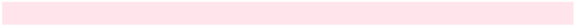
\includegraphics[keepaspectratio]{md/Aspose.Words.ef31fe30-39fd-431f-886c-9330939ce209.002.png}}}
  \end{itemize}
\end{itemize}

1.** QUÉ ES LA PSICOLOGÍA SOCIAL Y QUÉ HACE\pandocbounded{
\includegraphics[keepaspectratio]{md/Aspose.Words.ef31fe30-39fd-431f-886c-9330939ce209.003.png}}

Cómo y por qué las personas \textbf{piensan}, \textbf{sienten} y se \textbf{comportan} en las situaciones sociales, es decir, cuando hay una presencial \textbf{real, imaginaria o simbólica} de otras personas. De esta forma, investiga cómo están influenciados los entornos sociales en los que nos encontramos, por otras personas o por nuestros pensamientos sobre ellas.

\begin{enumerate}
\def\labelenumi{\arabic{enumi}.}
\tightlist
\item
  \textbf{La Psicología Social es una disciplina científica} El término \textbf{``ciencia''} alude a:
\end{enumerate}

\begin{itemize}
\tightlist
\item
  La adhesión a un conjunto de valores básicos → \emph{objetividad}
\item
  Al uso de métodos para estudiar sistemáticamente cualquier faceta del mundo
\end{itemize}

Existen cuatro valores básicos que motivan la actividad científica y hacen que esta pueda ser considerada como tal:

\begin{itemize}
\tightlist
\item
  \textbf{EXACTITUD}: adhesión del científico a una búsqueda y evaluación de la información sobre la realidad de forma rigurosa, precisa y que intenta apartarse de cualquier error.
\item
  La exactitud está ausente en la \textbf{observación espontánea} ya que es casual y se deja llevar por aquello que atrae nuestra atención.
\item
  \textbf{OBJETIVIDAD}: conseguir y evaluar la información relativa al objeto de estudio en sí mismo, con independencia de la forma de pensar o sentir de la persona que recoge esa información.
\item
  En la \textbf{observación espontánea} cada persona puede permitir que su forma de pensar o sentir contamine la información que observa.
\item
  \textbf{ESCEPTICISMO}: los resultados se aceptan solo si han sido verificados repetidamente (replicación).
\item
  \textbf{APERTURA MENTAL}: disposición para actualizar las conclusiones cando haya evidencia.
\end{itemize}

\begin{enumerate}
\def\labelenumi{\arabic{enumi}.}
\setcounter{enumi}{1}
\tightlist
\item
  \textbf{La Psicología Social se centra en el comportamiento de las personas}
\end{enumerate}

El comportamiento de las personas es lo que estudiamos, ya que es \textbf{observable} y puede ser \textbf{medido} \emph{(cuántos segundos tarda una persona en hacer una atribución de árabe-malo en comparación cuanto tarda en hacerla árabe-bueno). !{[}ref2{]}}

El comportamiento no se reduce \pandocbounded{
\includegraphics[keepaspectratio]{md/Aspose.Words.ef31fe30-39fd-431f-886c-9330939ce209.005.png}}\pandocbounded{
\includegraphics[keepaspectratio]{md/Aspose.Words.ef31fe30-39fd-431f-886c-9330939ce209.006.png}}

\texttt{}Observable y medible

únicamente a la \textbf{conducta motriz}

(caminar, saltar\ldots) sino también a Conducta motriz + expresiones

todo aquello que expresamos Motivaciones y metas

oralmente, por escrito o

gestualmente. Pensamientos, emociones, creencias, actitudes El comportamiento sirve para Procesos psicológicos subyacentes comunicar las \textbf{motivaciones} y Factores culturales o étnicos

\textbf{metas} que tienen las personas, así

\texttt{}Presencia de los demás

como sus pensamientos,

emociones, creencias y actitudes

que son directamente observables. En las situaciones en las que las personas no transmiten, éstos se pueden inferir a partir del comportamiento, es decir, pueden

ser deducidos.

Por otro lado, el comportamiento también hace referencia a los \textbf{procesos psicológicos subyacentes (cognitivos o emocionales),} no observables, que constituyen la dimensión psicológica del comportamiento.

Además, el comportamiento, los sentimientos y pensamientos se ven influenciados por \textbf{factores culturales y étnicos} y \textbf{la presencia de los demás}:

\begin{itemize}
\tightlist
\item
  \textbf{Física y real:} \emph{espectadores de un partiendo que alientan o abuchean.}
\item
  \textbf{Imaginada}: \emph{opositor ensayando su exposición frente a un tribunal imaginado.}
\item
  \textbf{Simbólica o implícita:} \emph{no te sientas en una silla porque hay una chaqueta y aunque la persona no está presente, nos abstenemos de ocupar ese sitio.}
\end{itemize}

La relación entre la conducta social y los procesos psicológicos subyacentes resulta \pandocbounded{
\includegraphics[keepaspectratio]{md/Aspose.Words.ef31fe30-39fd-431f-886c-9330939ce209.007.png}}de gran interés en los psicólogos sociales.!{[}ref2{]}

\bibliography{book.bib,packages.bib}

\end{document}
